%-----------------------
% Academic Research
%-----------------------

\chapter{Academic Research}
Research writing involves a number of critical skills: library research, 
critical thinking, the evaluation of sources, and the ability to synthesize 
information through summary, paraphrase, and quotation. Although synthesizing 
the thinking of others is an important part of the research essay, in its true 
form the research essay strives for much more than a mere re-presentation of 
what others have said on a particular topic or question. As \href{http://owl.english.purdue.edu/owl/resource/658/02/}{Jack Baker and Allen Brizee} state:

\begin{quote}A research paper is not simply an informed summary of a topic by 
means of primary and secondary sources. It is neither a book report nor an 
opinion piece nor an expository essay consisting solely of one's interpretation 
of a text nor an overview of a particular topic. Instead, it is a genre that 
requires one to spend time investigating and evaluating sources with the intent 
to offer interpretations of the texts, and not unconscious regurgitations of 
those sources. The goal of a research paper is not to inform the reader what 
others have to say about a topic, but to draw on what others have to say about 
a topic and engage the sources in order to thoughtfully offer a unique 
perspective on the issue at hand.\end{quote}

In high school you were perhaps asked to write research papers on predetermined 
topics. These essays were probably not what Baker and Brizee have in mind. Your 
projects were likely just retellings of what other scholars or writers have 
said on a topic. A true research essay involves blazing a new path of inquiry 
where you produce original ideas, questions and arguments. A research paper is 
a contribution to an ongoing conversation, a moment when you engage in dialogue 
with other important voices about a topic that you value.

\section{The Research Question}

Finding a research topic can be an overwhelming experience. With so many things 
to choose from, finding a narrow focus is often difficult. However, before you 
can truly begin your library research you need to find a way to narrow your 
field of inquiry to a single research question or problem.

At the outset your research questions will be rather general and mundane. But 
that is perfectly normal: we all have to start somewhere. Once you have a 
general topic of interest, however, you can move into a more rigorous research 
phase.

As you begin your research, try to keep an open mind and allow yourself to be 
pulled in new directions. It is important to think of the research process as 
something more than a mere attempt to find information on a predetermined 
topic. Research is also a process of discovery where you encounter ideas and 
contemplate questions that you would have otherwise never imagined. 

\section{Finding A Topic}
\subsection{Exploring Topics with Subject Searches}
If you are having difficulty finding a narrow topic of interest, one way to get 
started is to examine an organized list of \emph{every} subtopic that is 
related to your broader subject. Since the 
\href{http://catalog.loc.gov}{\{Library of Congress\}} assigns a series of 
\textbf{subject headings} to every published book, you can easily browse a 
meticulously categorized list of books that relate to your broader research 
subject. For example, if you want to write an essay on the nation of Iraq, you 
can perform a subject search with the search term "Iraq." The result will be an 
alphabetized list of \emph{every} subject that scholars have written on about 
Iraq\textemdash from agriculture to zoology. So, if you haven't yet found a 
narrow focus for your project, you can use the subject headings to "shop" for a 
subject that interests you. 

\subsection{Finding Additional Sources through Subject Searches}
Subject searches are also a helpful means of finding additional sources on your 
topic once you have acquired one or more. For example, if you discover that 
historian Alan Taylor's book, \emph{The Civil War of 1812}, is an important 
source for your research project, you can use the book's subject headings to 
find all of the other books written on those topics. The Library of Congress 
assigned the book the following three subject headings:

\begin{quote}
United States--History --War of 1812 --Social aspects

Ontario--History --War of 1812 --Social aspects

Northern boundary of the United States--History--19th century
\end{quote}

In most library catalogs these subject headings are hyperlinked; clicking on 
any of them leads you to a list of every other book in the library that shares 
that particular subject heading. Thus, if your research interest is 
\textbf{United States -- History -- War of 1812 -- Social aspects}, you can 
quickly find every other book on that subject with a subject search. 

Though Mugar's holdings are not nearly as large as the Library of Congress, you 
can perform subject searches by using the 
\href{http://buprimo.hosted.exlibrisgroup.com:1701/primo_library/libweb/action/s
earch.do?dscnt=1&scp.scps=scope%3A%28BOSU%29%2Cscope%3A%28BU_OAI%29%2Cprimo_cent
ral_multiple_fe&tab=default_tab&dstmp=1359630002248&vid=BU&mode=Advanced&fromLog
in=true}{\{Advanced Search\}} feature of our library catalog.

\section{Finding Background Information}

A research project should always begin with the reading of general background 
information about the topic. Before you can ask an intelligent question about 
your topic or contribute to an ongoing scholarly conversation, you need to 
develop a working knowledge of basic facts to serve as a foundation for your 
project. The best way to develop this basic understanding is to examine 
peer-reviewed reference works, such as encyclopedias.

Mugar library has a number of helpful reference resources in this regard. If 
you visit the 
\href{http://www.bu.edu/library/research/guides/research-guides}{\{Library 
Research Guides\}} link on the \href{http://www.bu.edu/library}{\{Mugar 
Homepage\}}, you will find an impressive array of organized reference materials 
like bibliographies, encyclopedias and dictionaries. Most of them are fully 
digitized and do not even require a trip to the library. Always start your 
research project with reference works and gain a basic grounding of your topic 
before developing your research question or thesis.

Other helpful background information aids of note:

\begin{itemize}
\item \href{http://www.wikipedia.org}{\{Wikipedia\}}

\item \href{http://www.cia.gov/library/publications/the-world-factbook/}{\{CIA 
World Factbook\}}

\item \href{[http://www.oxfordreference.com.ezproxy.bu.edu}{\{Oxford Reference 
Online\}}

\end{itemize}
A word of warning about Wikipedia (and internet sources in general): it has not 
been through a process of peer review. For that reason, it is unwise to use 
Wikipedia as a source for a research project. In addition, many professors will 
refuse to accept Wikipedia as a legitimate source. 

\section{Searching for Books}

Mugar library provides both \href{http://www.bu.edu/library}{\{simple\}} and 
\href{http://buprimo.hosted.exlibrisgroup.com:1701/primo_library/libweb/action/s
earch.do?tab=default_tab&mode=Advanced&scp.scps=scope%3a%28BOSU%29%2cscope%3a%28
BU_OAI%29%2cprimo_central_multiple_fe&vid=BU}{\{advanced\}} searching of the 
library catalog. The simple search feature provides you with an experience 
similar to Google. You can enter an author's name, the title of a book, or 
keywords. Once the search results are presented on the screen, use the "Refine 
my Results" links on the left of the page to limit the search to "print books" 
or "electronic books."

\section{Searching for Periodicals/Articles}

Periodicals are publications that are published at regular intervals, such as 
scholarly journals, magazines and newspapers. Examining periodicals\textemdash 
especially academic journals\textemdash is an important aspect of research. 
Since books often take a year or more to go through the process of peer review, 
editing, typesetting and printing before they become available for purchase, 
they often do not contain the most current information. Articles, on the other 
hand, appear in a far shorter period of time and generally contain the most 
up-to-date research. For that reason, you should perform a review of journal 
articles on your research topic to ensure that you are aware of recent 
discoveries, arguments, and debates within the academic community who share 
your research focus.

The librarians at Mugar library have created a convenient 
\href{http://www.bu.edu/dbin/ejournals/esources/alpha-es.php}{\{Periodical 
Index\}} that lists each of our periodical databases alphabetically. If you 
know the name of a particular journal or database, you can select it from the 
index and begin searching for information.  

However, a common problem for undergraduate researchers is not knowing which 
databases or journals to search for information on a particular topic. Unless 
you are a professional scholar, it is difficult to know what the leading 
journals are in a particular field of study. Although an English professor 
would know that the academic journal \emph{PMLA} or the database JSTOR are 
excellent places to look for articles on Herman Melville's novel, \emph{Moby 
Dick}, the novice research wouldn't know where to begin. 

To resolve this problem, our library has authored a broad collection of 
\href{http://www.bu.edu/library/research/guides/research-guides}{\{Research 
Guides\}} designed to help you locate the specific journals, periodical 
databases, and reference materials that are appropriate for each discipline or 
research topic. These are an indispensable resource for discovering 
peer-reviewed sources on your chosen topic. 

\section{Searching with Precision}

A common research problem is that your searches produce too many results. 
Rather than page through hundreds or thousands of search results, you should 
become familiar with powerful \textbf{Boolean searches} to make your search 
terms more precise. Boolean searches use what are known as \textbf{logical 
operators} to form search terms. The three most common logical operators are 
AND, OR, and NOT. 

\subsection{AND}

Although it may seem counterintuitive, \textbf{AND} functions to \emph{limit or 
narrow} the number of sources you retrieve from a database. You can visualize 
the search of a large academic database or library catalog using the following 
diagram:
 
\begin{center}
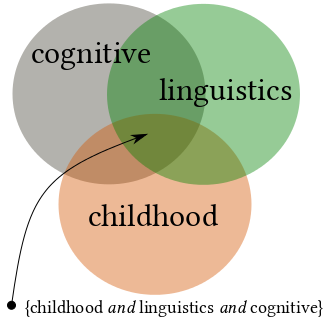
\includegraphics[width=.45\textwidth]{and3colors.png}
\end{center}

In the search depicted above, a student has requested articles that contain the 
subjects \textbf{cognitive}, \textbf{linguistics}, and \textbf{childhood}. 
Significantly, this particular search will only retrieve articles that contain 
\emph{all three terms}. This small subset of the larger subject sets is 
referenced by the arrow. All the information represented by the other portions 
of the three circles will be excluded. Thus, even if an article contains two of 
the three search terms, it will be excluded from the results.

\subsection{OR}
Unlike the \textbf{AND} operator, \textbf{OR} seeks to \emph{broaden} a search, 
as in this example:

\begin{center}
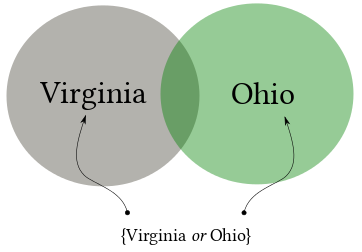
\includegraphics[width=.45\textwidth]{Orcolor.png}
\end{center}

In the search depicted above, a student has searched for the subjects Virginia 
\textbf{OR} Ohio. This search will return \emph{every} article having the 
subject of Virginia as well as \emph{every} article with the subject of Ohio. 
Unlike the \textbf{AND} search, where only articles containing \emph{both} 
terms are returned in the search results, the \textbf{OR} search yields every 
article on both subjects regardless of whether those subjects appear together 
in the same article. As a consequence, the \textbf{OR} search will produce far 
more results. 

Since the \textbf{OR} operator lacks precision, it is most often used in 
parenthetical searches, described below.

\subsection{NOT}
The Boolean operator \textbf{NOT} is used to \emph{subtract} or \emph{screen 
out} topics or keywords that are unwanted within the search results. 


\begin{center}
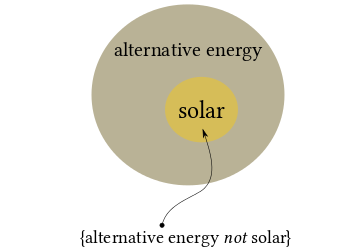
\includegraphics[width=.45\textwidth]{notcolor.png}
\end{center}


In the search depicted above, a student is researching alternative energy and 
wants to exclude any information dealing with solar energy. To remove all 
references to solar energy, the student has searched for \textbf{alternative 
energy}, but has removed any articles from the search results that contain the 
subject \textbf{solar} using the operator \textbf{NOT}. 

The \textbf{NOT} operator is helpful when you find your search results are 
"polluted" with unwanted items. This is often a problem when two distinct 
things share the same name. For example, if you were researching the Norse 
explorers known as the Vikings, you might discover that your search results 
include unwanted information about the Minnesota Vikings football team. You can 
subtract these unwanted results by searching for \textbf{Vikings not Minnesota} 
or \textbf{Vikings not football}.  

\subsection{Parenthetical Searches}

You can also use the various Boolean search terms in tandem using parenthetical 
constructions:

\begin{itemize}
\item (Ohio or Virginia) and unemployment
\item (cognitive and linguistics) not childhood
\end{itemize}
Such parenthetical searches follow the order of operations, like in math 
equations. In the first example, the search will first combine all the articles 
that are on the subjects of \textbf{Ohio} or \textbf{Virginia}, creating a 
large collection of search results. Afterward, the search term 
\textbf{unemployment} will be applied to that collection, yielding the final 
search results. Similarly, the second example creates a large collection of 
results that share the subjects \textbf{cognitive} and \textbf{linguistics}, 
then all the items having the subject \textbf{childhood} are removed from the 
results.

\subsection{Exact Phrase}

Most Internet search engines and library catalogs default to the \textbf{AND} 
operator when multiple terms are entered, even if it has not been typed by the 
user. For example, if you search for \textbf{artificial intelligence}, the 
search algorithm will actually use the search phrase \textbf{artificial 
\emph{and} intelligence} to produce your results. In some circumstances this 
may produce undesirable or imprecise results.

To avoid this problem, you can instruct your search engine to perform what is 
known as an \textbf{exact phrase search}. This is performed by placing 
quotation marks around the exact words that you are searching for. By searching 
for "artificial intelligence" your search results will only contain items that 
have that exact phrase within the document.

\subsection{Truncation and Wild Cards}
\begin{itemize}
\item manufact\** [truncation]
\item wom\**n [wild card]
\end{itemize}
If you search for the terms \textbf{steel and manufacturing}, your search 
results will not include results with the terms \textbf{manufacturer}, 
\textbf{manufacture}, \textbf{manufactured}, or \textbf{manufactures}. As a 
result, you may not discover articles or books that are important to your 
research. By truncating the word with an asterisk, you will gather all the 
relevant search results. 

Similarly, if you only search for wom\underline{en}, you will miss out on the 
all the texts that mention wom\underline{an}. However, using the wild card 
asterisk you will search both terms simultaneously.

\section{Finding a Book in the Library}

\subsection{The Library of Congress System}
Most research libraries use the Library of Congress (LC) classification system 
to organize their holdings. The Library of Congress assigns each book a unique 
\textbf{call number} consisting of a series of numbers and letters that help 
you locate them on the library's shelves. A typical call number will resemble 
the following: 

\begin{quote}
\hspace{.4in}{\huge F 24 .T39 1990}
\end{quote}

Let's break down the call number into its component parts:

\begin{quote}
\hspace{.4in}\begin{tabular}{ |l|l| }
  \hline
  F & Letter, or subject, line \\ \hline
  24 & Whole number line \\
  \hline
  .T39 & Cutter line \\ \hline
  1990 & Edition, or Date, line\\ \hline
\end{tabular}
\end{quote}

\begin{itemize}
\item \textbf{The Letter line} describes the subject matter, or discipline, of 
the book. It also indicates the section of the library where the book is 
shelved (consult your library's map and floorplan). The letter line will be 
between one and three letters long.
\item \textbf{The Whole number line} tells you which \emph{row} the book is on 
in the stacks. 
\item \textbf{The Cutter line} identifies the \emph{individual book}. The first 
letter of the Cutter line is usually the first letter of the author's last name.
\item \textbf{The Edition, or Date, line} tells you the book's year of 
publication. This line is used to distinguish between editions.
\end{itemize}

\subsection{How to Find a Book}
To find a book in the library, read the call number from left to right, using 
alphabetical and numerical orders. First, using the \textbf{Letter line}, 
determine the floor of the library where the book is shelved. Use the library's 
\href{http://www.bu.edu/library/mugar-memorial/about/floorplans/#f=floor-1}{\{fl
oorplan maps\}} to locate the proper section. Using our example call number 
above, we can determine that the \textbf{F} section is on the 4th floor of 
Mugar library. 

Once on the appropriate floor, use the \textbf{Whole number line} to find the 
row where the book is shelved in the stacks. Using the example call number, we 
will look through the stacks for the number 24. The floormaps are often helpful 
in locating the book's general location on the library floor. As you walk 
through the stacks, look on the ends of each row of books for signs describing 
the range of books held within the rows. You might, for example, see a sign 
reading:

\begin{center}
\hspace{.4in}{\huge F 7.4\textendash F 45.2}
\end{center}

Since \textbf{F 24} is within this range, our example book is in that row. Once 
in the proper row of shelves, proceed numerically until you find the 24s. 

Finally, using the \textbf{Cutter line}, proceed alphabetically until you find 
the Ts. Then proceed numerically until you find .T39, the address of our book. 

As you can see, the call number should be read from left to right using 
alphabetical and numerical orders. Thus, a book with a Subject line \textbf{F 
}would be shelved \emph{before} a book with a Subject line \textbf{FA.} 
Similarly, a Cutter line that reads \textbf{.T39} is shelved \emph{after} 
\textbf{.T21}. 

\begin{itemize}
\item \textbf{Remember, in decimals .7 is bigger than .21!}
\end{itemize}

Maps of the library's floorplans are affixed to the walls on each floor. Free 
paper maps of the library are available at the circulation desk of the library. 
You may also consult the 
\href{http://www.bu.edu/library/mugar-memorial/about/floorplans/#f=floor-1}{\{ma
ps and floorplans\}} online or with your computer or smartphone. 

\section{What if we don't have it?}
    
A common problem in academic research is discovering that a source that you 
require for a project is checked out, missing, or not owned by the library. 
There are a number of free services available to you when you encounter this 
problem.

\subsection{Boston Consortium Libraries}

A number of Boston-area colleges and universities have formed a library 
consortium designed to share resources and expand research options for the 
entire academic community. As students of Boston University, you may obtain 
borrowing privileges at any of the other participating libraries. 

To see if a book is available at another 
\href{http://www.blc.org/members/current-members}{\{BLC\}} library, use a 
service called \href{http://www.bu.worldcat.org}{\{WorldCat Local\}}. With this 
service you can search every library in the BLC simultaneously to see if the 
book you require is available at another local institution. If the book is 
owned by another school and is not checked out at the time, you may request 
that the item be sent to our library. To request a book, browse to the book's 
record in the WorldCat catalog and click the green button labeled "Request 
Item." Once Mugar's circulation desk receives the item, they will inform you 
through email that the text is ready for pickup.

\subsection{Boston Library Consortium Card}
If you would like to check out a book at one of the other BLC member libraries 
in person, you may obtain borrowing privileges by applying for a 
\href{http://www.bu.edu/library/services/ill/blc-cards}{\{Boston Library 
Consortium Card\}}. To apply, fill out the online form and you will be 
contacted when your card is ready for pickup at Mugar's circulation desk.

\subsection{Interlibrary Loan}
If there is a book or article you would like to read that is not available at 
any BLC library, you may request it from BU's Interlibrary Loan office. To 
request an item, visit the 
\href{http://illiad.bu.edu/illiad/bos/illiad.dll}{\{Interlibrary Loan\}} 
webpage, select the appropriate form (article, book, book chapter, etc.), and 
send your request electronically to the ILL office. The staff in the office 
will request your item from another library, who will ship the book to our 
library through the mail. 

\textbf{Please note}: Interlibrary Loan is the \emph{slowest} of all the 
available options for requesting research materials. Requests may take up to 
two weeks to be fulfilled. 


\section{Research Guides}

If you are performing research on a topic and do not know where to begin, 
Boston University Librarians have created an impressive collection of 
\href{http://www.bu.edu/library/guides/index-a-h.html}{\{Research Guides\}} 
that can help you find background information, periodical databases, and 
academic journals appropriate for your topic or discipline:

\begin{itemize}
\item\href{http://www.bu.edu/library/research/guides/research-guides/area-and-cu
ltural-studies/}{\{Area and Cultural Studies\}}
    
\item\href{http://www.bu.edu/library/research/guides/research-guides/arts-and-hu
manities/}{\{Arts and Humanities\}}

\item\href{http://www.bu.edu/library/research/guides/research-guides/management-
business/}{\{Business and Management\}}

\item\href{http://www.bu.edu/library/research/guides/research-guides/science-and
-engineering/}{\{Science and Engineering\}}

\item\href{http://www.bu.edu/library/research/guides/research-guides/social-scie
nce/}{\{Social Sciences\}}
\end{itemize}

\section{Peer Review}

Peer review is a form of quality control in academic publishing. Before books 
or articles are published, they experience a rigorous process of evaluation by 
a number of experts who have advanced training in the field of study in 
question. This scholarly review helps eliminate factual errors and other 
problems before the works are published. Thus, peer-reviewed works much more 
trustworthy than other sources of information. 

\subsection{How do you determine if a source is peer-reviewed?}

For novice researchers, distinguishing between peer-reviewed and other kinds of 
sources can be challenging. 

There are a number of things you can do to ensure that you are using 
peer-reviewed information. Many periodical databases, such as 
\href{http://www.jstor.org.ezproxy.bu.edu/jstor/}{\{JSTOR\}}, only contain 
peer-reviewed academic articles. Many other databases, such as 
\href{http://infotrac.galegroup.com.ezproxy.bu.edu/itweb/mlin_b_bumml?db=AONE}{\{Academic OneFile\}}, have a search limiters that can be selected to ensure 
that the search results only contain peer-reviewed sources. However, other 
databases lack clear indications about the nature of their sources. If you are 
confused about a source or database, ask your professor or one of the research 
librarians for assistance.

If those are not practicable, use these test criteria:
\begin{itemize}
\item Scholarly, peer-reviewed articles almost always publish the university 
affiliation of the professor/author/scientist. 

\item Scholarly articles \emph{always} have a bibliography page. 

\item Scholarly articles always contain citations and commonly have footnotes 
or endnotes. 

\item Generally speaking, if you can find the publication at the dentist's 
office or on an airport magazine rack, then it isn't scholarly or 
peer-reviewed. \emph{Time}, \emph{Newsweek}\textemdash even the \emph{New York 
Times}\textemdash are not considered peer-reviewed sources.
\end{itemize}

\section{The Oxford English Dictionary}

The \href{http://www.oed.com.ezproxy.bu.edu}{\{OED\}} is, without question, the 
greatest and most complete dictionary ever created. Many generations of 
scholars have made it their life's work. The OED systematically traces the 
etymology of words in the English language. 
\href{http://en.wikipedia.org/wiki/Etymology}{\{Etymology\}} is "the study of 
the history of words, their origins, and how their form and meaning have 
changed over time." Thus, with the OED you can see when a word entered or 
exited the English language and how its meaning evolved over time. 

The OED is quite helpful when you are reading a novel, poem, or document that 
was written in a time period distant from our own. Since words fall out of use 
and the meanings of words change over time, it can often be difficult to 
interpret the meaning of the texts we read from the past. The OED exists to 
help us with this problem: you can think of it as a dictionary with a built-in 
time machine. 


\section{Helpful Research Suggestions}

\subsection{Not all sources are equal}

How do you know if you can trust your source? Here are some suggestions for 
critically examining your sources:

\begin{itemize}
\item \textbf{Examine the credentials of the author}. What is their educational 
background? Do they have an advanced degree in the subject that they are 
writing about? Are they affiliated with any major institutions\textemdash such 
as a university or government department? Does the author have a respected 
publication record that is frequently cited by other experts in the field?

\item \textbf{Examine the date of publication}. When was the book or article 
you are reading published? Since new discoveries and ideas are produced every 
day, it is important to consult the most recent sources on your research 
subject. Generally, the most current source should be preferred over older 
sources.

\item \textbf{Determine if the source has been peer-reviewed}. Peer review is a 
form of quality control in academic publishing. It ensures that the information 
that is published has been properly evaluated and vetted by a number of other 
professionals in the field. A peer-reviewed source should be preferred over any 
other kind of information.

\item \textbf{Be wary of Internet sources}. If your source comes from the 
Internet, you should take care to verify its trustworthiness. Most sites on the 
Internet are not peer-reviewed sources of information. Misleading, politically 
motivated, and even propagandistic content often masquerades as objective 
information on blogs, websites, and discussion boards. 
\end{itemize}

\subsection{Taking notes}

Now that you have some research materials in front of you, either at the 
library or at home, it's time to make them useful to you. Before placing source 
materials in your essay, take good notes instead by using summary, paraphrase, 
and judicious quotation to take ownership of the source materials. Ensure that 
you cite appropriately and that your summaries and paraphrases use your own 
original language. This intermediary step before writing the essay saves you 
time and helps you avoid plagiarism.

If you'd keep organized notes on your computer, try the free, open-source 
program called \href{http://rasm.ods.org/keepnote}{\{Keepnote\}}.

\subsection{Raid the Bibliography}

Occasionally, students find one or two sources on a topic and then despair of 
finding any more. However, with just one excellent article or book, you can 
easily generate additional research leads. When you find a book or article that 
relates to your project, scour the bibliography to see what books and articles 
the author used to produce his or her work. Make lists of the most promising 
sources by writing down all the bibliographic information in a research 
journal. Locate these sources in the library and then repeat the process. By 
using this technique of routinely following up on sources cited in 
bibliographies, you can generate a surprisingly large number of books and 
articles on your topic in a relatively short time.

\subsection{Keep a Research Journal}

Keeping a research journal is an important habit to develop. Every student or 
professor has had the unsettling realization that they have used a quotation in 
their writing but have no recollection of where the quote came from. Many hours 
can be consumed retracing steps. Frequently, source materials are never located 
again. To avoid this problem, keep a research journal where you record the 
bibliographic information of each source you read or browse. This way you can 
quickly locate the information again. 

Although a paper notebook works well as a research journal, there are some very 
promising electronic alternatives. This bibliographic software can maintain a 
record of your sources, help you take notes, and even produce perfectly 
formatted bibliography pages for your essays. 

For Mac users, there is \href{http://www.sonnysoftware.com/}{\{Bookends\}}. PC 
users should consider \href{http://www.biblioscape.com}{\{Biblioscape\}}. 
However, the free and open-source option known as 
\href{http://zotero.org}{\{Zotero\}} is perhaps the best option of all.

